\section{Introduction}\label{sec:intro}

With the long-term research on emotion theory from psychology and neuroscience\cite{james1884emotion, turkle2005second}, emotion has been confirmed to be a significant effect \cite{james2013emotion} on human communication, decision making, perception and so on.

Affective computing is an emerging interdisciplinary research field ranging from computer vision, machine learning, nature language understanding and human computer interaction (HCI), as well as cognitive and social sciences.

On the perspective of human computer interaction, Picard \cite{Picard1999} pointed out that affective computing involved projects can be used for \emph{reducing user frustration enabling comfortable communication of user emotion}, \emph{developing infrastructure and applications to handle affective information}, as well as \emph{building tools that help develop social-emotional skills}.

% 2. 然后介绍人类情感的表达方式,以及它们可能通过哪些信息进行采集。\cite{Hertenstein2009} 这篇文章有一副图片非常详细描述了不同的人类情感及其相关表达部位,同时还包含了不同性别之间的差异。

% 历年来有两篇 \cite{Zhang2014, Politou2017} 有介绍了关于 smartphone sensor 的问题。但是并没有对具体的技术进行相关介绍,同时存在大量的内容丢失;

% 一篇 \cite{Garcia-Garcia2017} 详细探讨了普世计算下的 unimodal analysis 到 multimodal analysis,全面分析了不同数据类型之间的结合以及它们所使用的方法,但是并没有考虑传感器ABC,同时它们得出的一些比较好的方法并不一定使用移动设备。

Figure~\ref{fig:hierarchically} shows the hierarchically-structured taxonomy of this paper.
In the following sections, we first  how recent researches involve different mobile commodity sensors to inferring user emotions in Section~\ref{sec:source}. 

\begin{figure}[H]
    \centering
    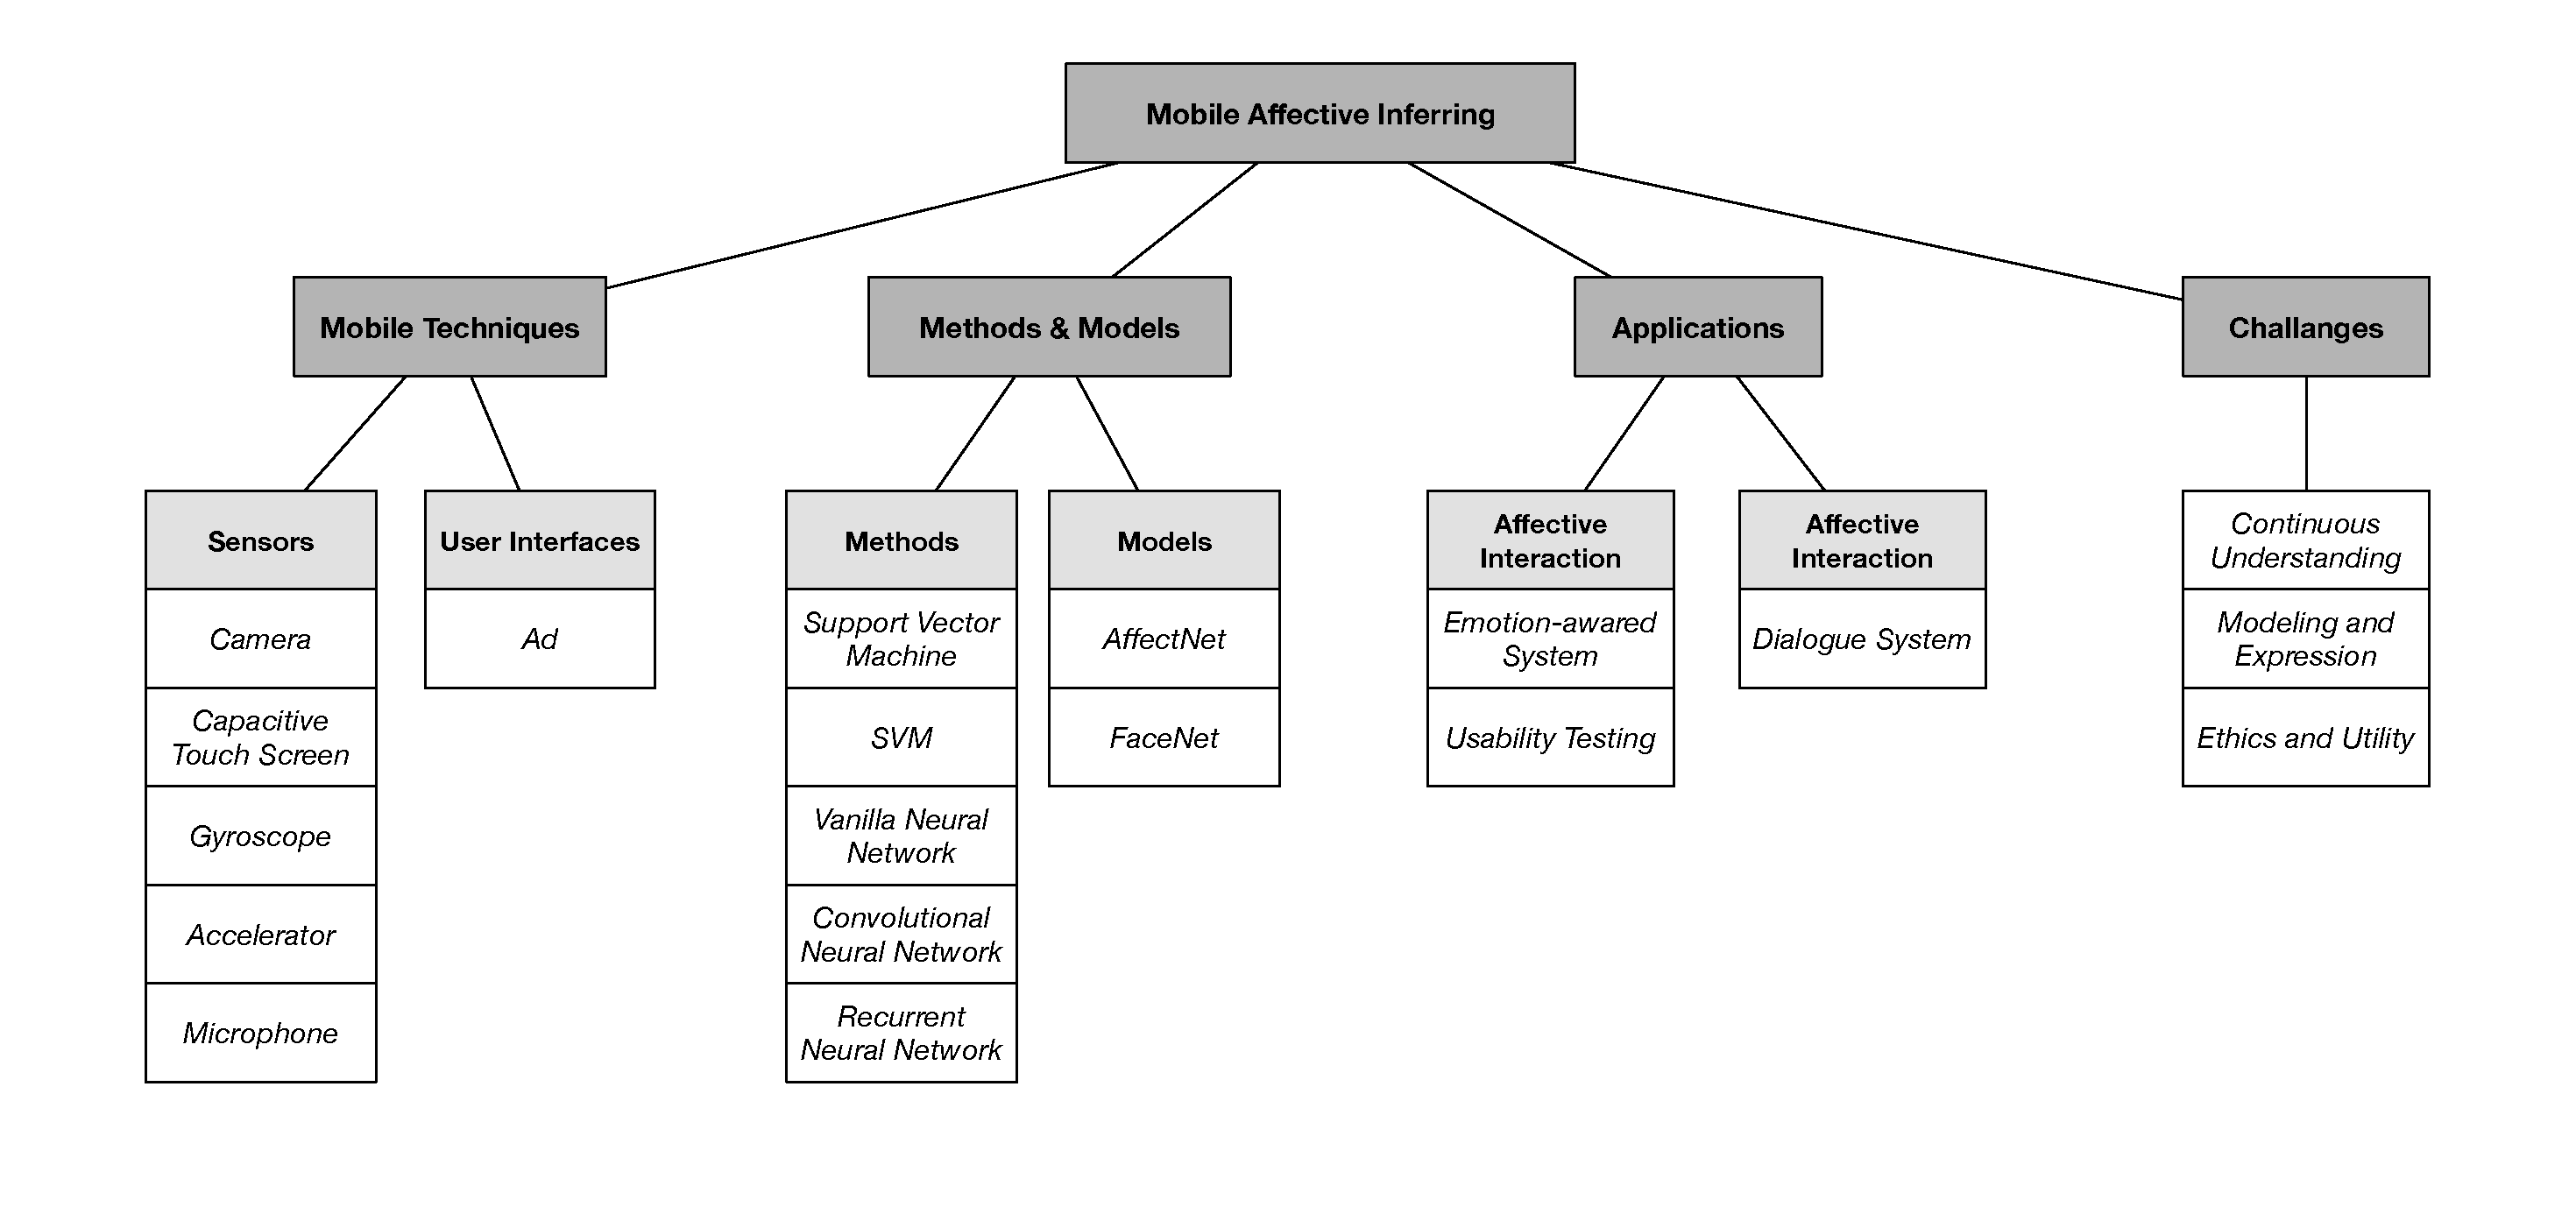
\includegraphics[width=0.5\textwidth]{hierarchical}
    \caption{Hierarchically-structured taxonomy of this paper.}
    \label{fig:hierarchically}
\end{figure}